\section{Diagrammi di attività}
In seguito vengono descritte le interazioni dell'utente con MaaS utilizzando i diagrammi di attività, secondo la seguente struttura:
\begin{itemize}
\item \textbf{Utente non autenticato};
\item \textbf{Utente autenticato};
\item \textbf{Super admin}.
\end{itemize}
\subsection{Utente non autenticato}
\begin{figure}[H]
\begin{center}
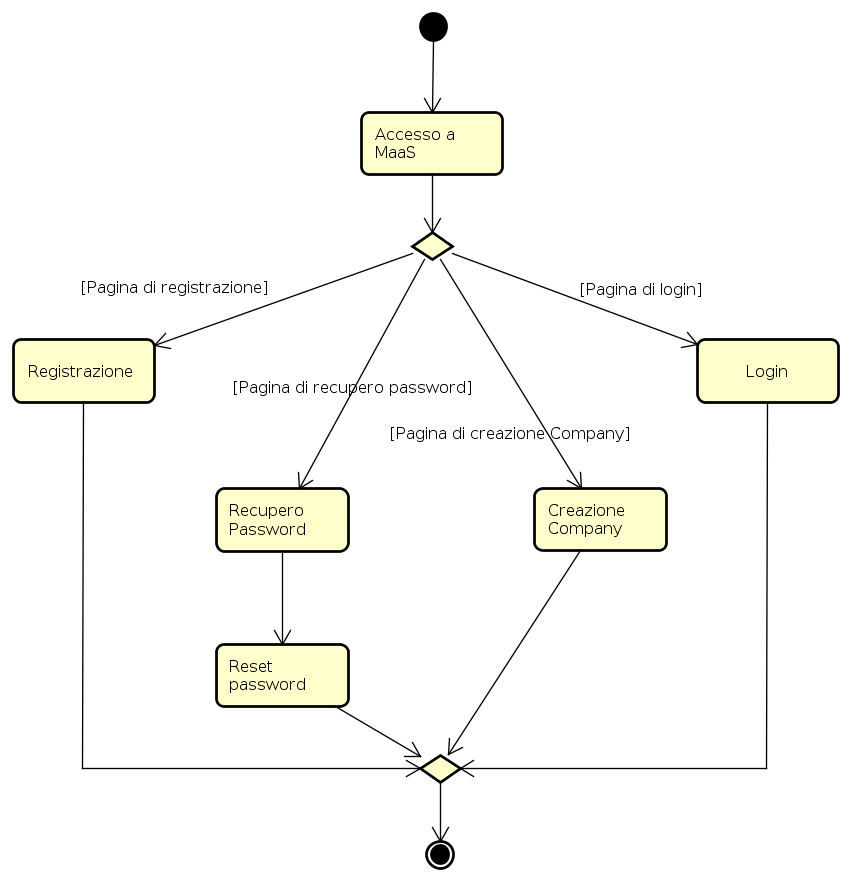
\includegraphics[height=12cm]{res/sections/backend/activities/principaliSenzaAuth.png}
\caption{Attività principali per un utente non autenticato}
\end{center}
\end{figure}
Un utente non autenticato, una volta visualizzata la pagina di MaaS, può:
\begin{itemize}
\item registrarsi, a seguito di un invito di un owner di una company;
\item effettuare il login;
\item eseguire la procedura di recupero password;
\item creare una nuova Company. L'utente verrà registrato come owner della company appena creata.
\end{itemize}
\subsubsection{Registrazione}
\begin{figure}[H]
\begin{center}
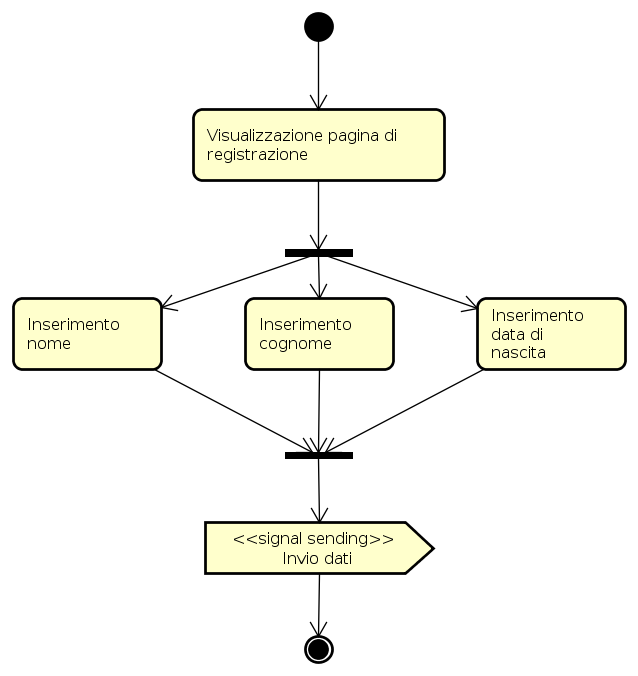
\includegraphics[height=12cm]{res/sections/backend/activities/registrazione.png}
\caption{Registrazione a MaaS}
\end{center}
\end{figure}
L'utente si trova nella pagina di registrazione a MaaS. Indirizzo email e password sono già stati impostati, e potrenno essere modificati dopo il completamento della procedura di registrazione; viene richiesto l'inserimento di tre campi base per il profilo di un utente: nome, cognome e data di nascita.
\subsubsection{Login}
\begin{figure}[H]
\begin{center}
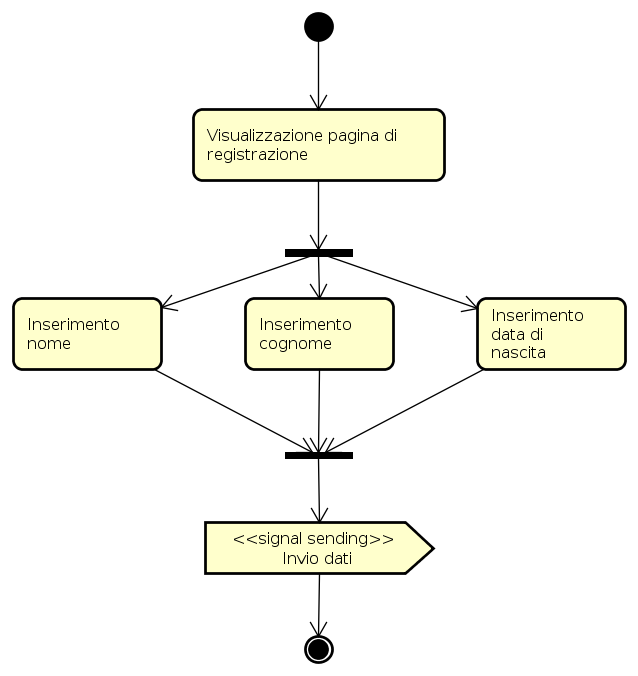
\includegraphics[height=12cm]{res/sections/backend/activities/registrazione.png}
\caption{Login}
\end{center}
\end{figure}
L'utente non autenticato deve inserire, in due caselle di testo, le proprie credenziali di accesso, username e password, per poter accedere a MaaS. Se le credenziali risultano valide l'utente veràà reindirizzato alla pagina contenente la propria dashboard, altrimenti verrà mostrato un messaggio di errore.
\subsubsection{Recupero password}
\begin{figure}[H]
\begin{center}
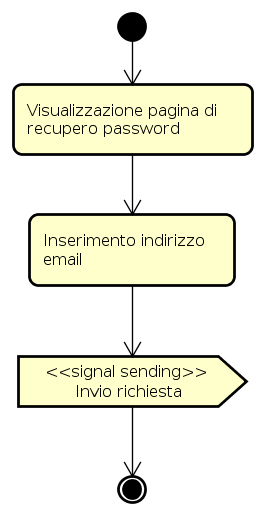
\includegraphics[height=12cm]{res/sections/backend/activities/recuperoPassword.png}
\caption{Recupero password}
\end{center}
\end{figure}
L'utente non autenticato deve inserire, in una casella di testo, l'indirizzo email al quale sarà inviato il codice segreto da utilizzare nella procedura di reset della password.
\subsubsection{Reset password}
\begin{figure}[H]
\begin{center}
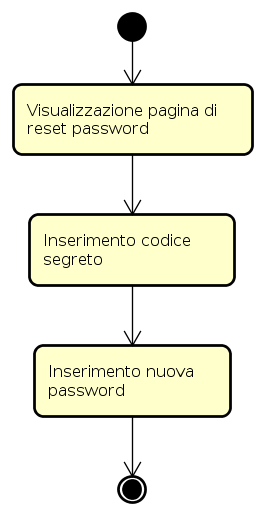
\includegraphics[height=12cm]{res/sections/backend/activities/resetPassword.png}
\caption{Reset password}
\end{center}
\end{figure}
L'utente non autenticato deve inserire, in una casella di testo, il codice segreto che ha ricevuto tramite email necessario a eseguire il reset della password. Se il codice è verificato, l'utente non autenticato potrà inserire una nuova password, che verrà memorizzata al posto della vecchia.
\subsubsection{Creazione company}
\begin{figure}[H]
\begin{center}
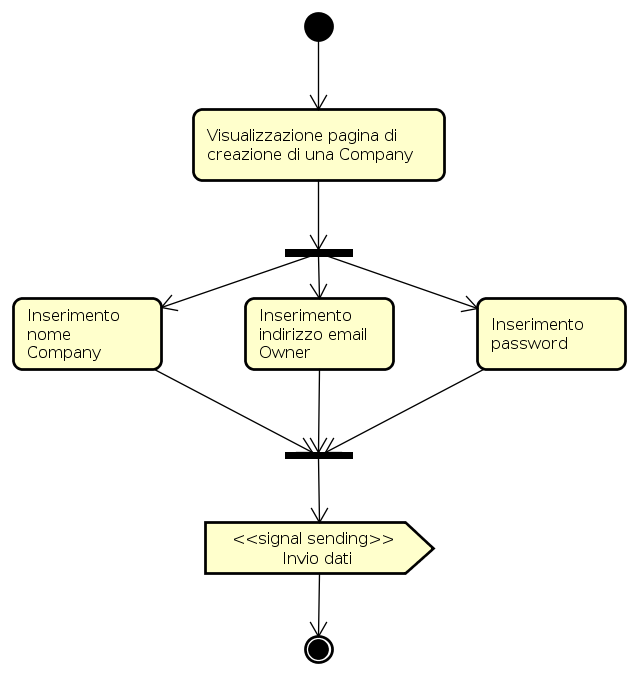
\includegraphics[height=12cm]{res/sections/backend/activities/creazioneCompany.png}
\caption{Creazione company}
\end{center}
\end{figure}
L'utente non autenticato che crea una company viene registrato come suo owner. È pertanto necessario fornire, durante la procedura di creazione, l'indirizzo email e la password dell'utente, oltre che il nome della company stessa.
\newpage
\subsection{Utente autenticato}
\begin{figure}[H]
\begin{center}
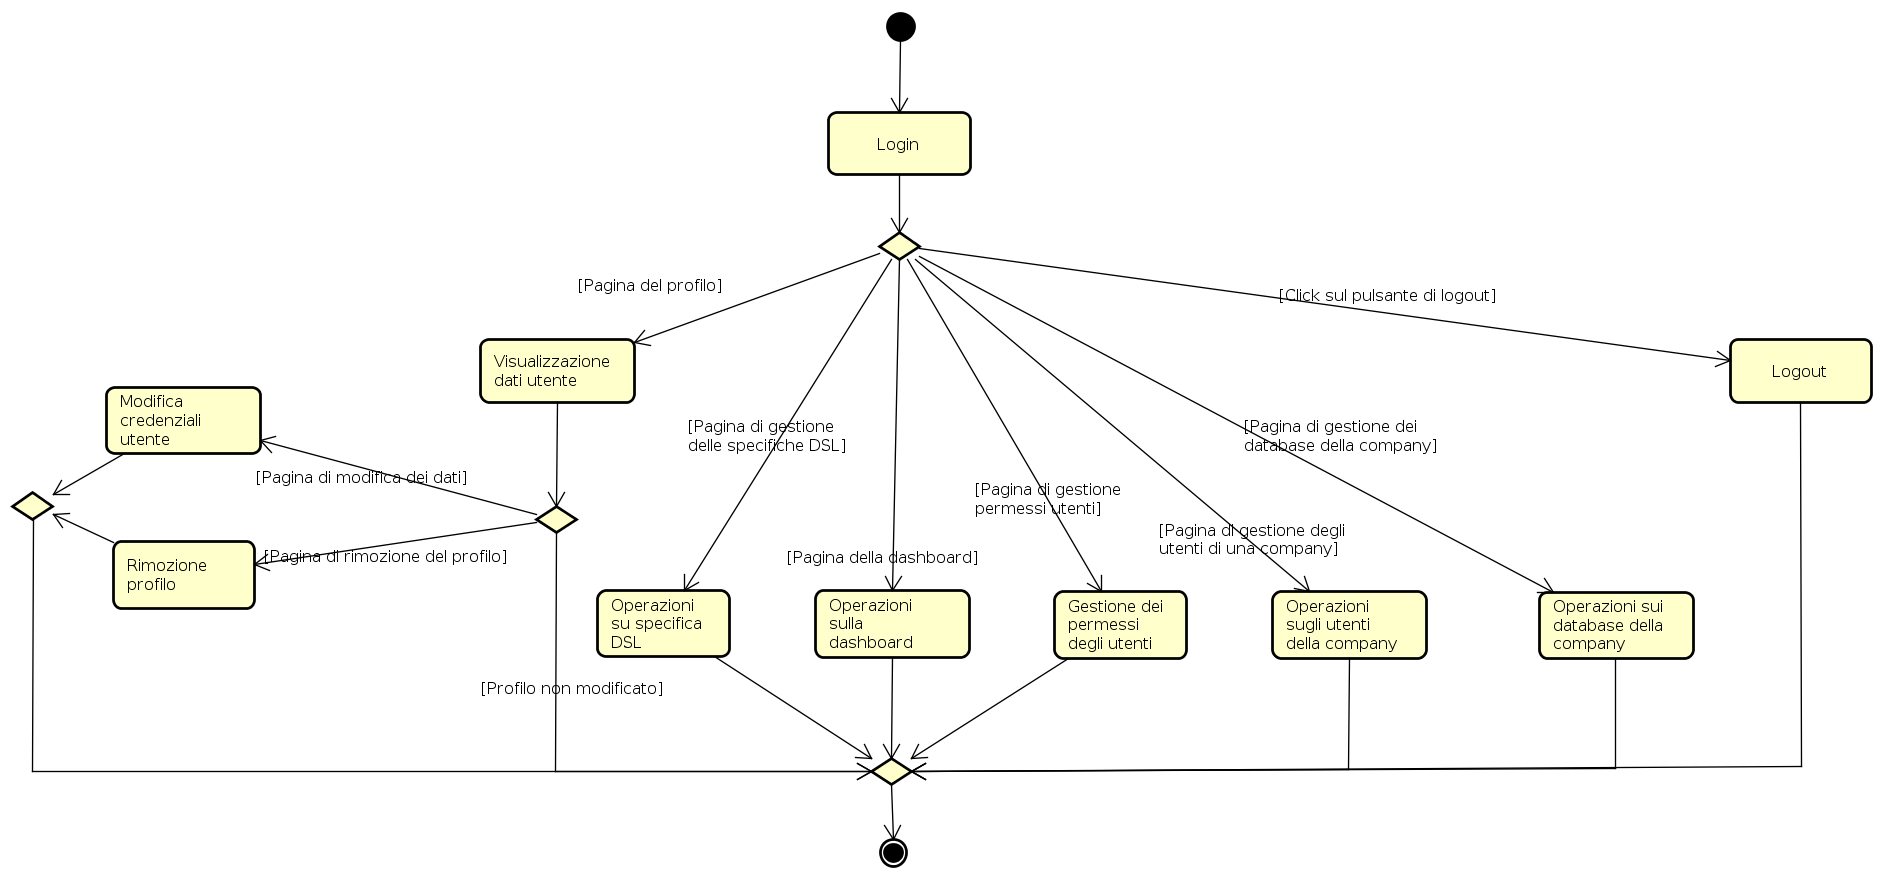
\includegraphics[width=18cm,angle=90]{res/sections/backend/activities/principaliConAuth.png}
\caption{Attività principali per un utente autenticato}
\end{center}
\end{figure}
Dopo aver effettuato il login un utente può:
\begin{itemize}
\item visualizzare le proprie credenziali di accesso, modificarle o rimuoversi da MaaS;
\item eseguire operazioni che coinvolgono specifiche DSL;
\item eseguire operazioni sulla sua dashboard;
\item gestire i permessi degli altri utenti (solo per admin e owner);
\item gestire gli utenti della company(solo per admin e owner);
\item visualizzare e gestire (quest'ultima solo per admin e owner) i database della company;
\item effettuare il logout.
\end{itemize}
\subsubsection{Modifica delle credenziali utente}
\begin{figure}[H]
\begin{center}
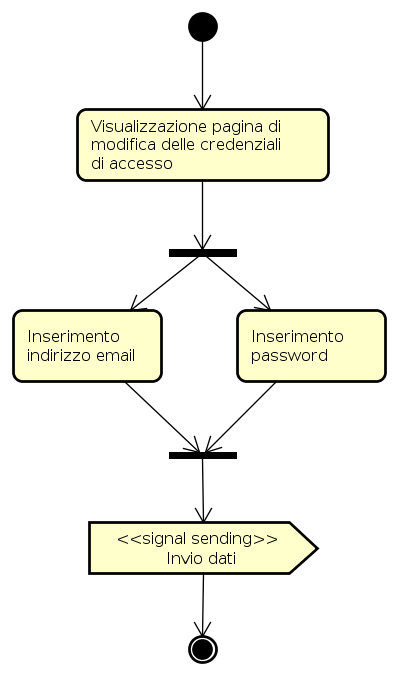
\includegraphics[height=12cm]{res/sections/backend/activities/modificaCredenziali.png}
\caption{Modifica delle credenziali utente}
\end{center}
\end{figure}
L'utente autenticato, dopo aver visualizzato la pagina con i suoi dati personali, può decidere di modificare le proprie credenziali di accesso inseremdo email e passowrd. Nel caso in cui le credenziali non siano valide (ad esempio, in caso di inserimento di un indirizzo email già presente) verrà visualizzato un messaggio di errore nel momento di invio della richiesta di modifica.
\subsubsection{Rimozione dell'utente}
\begin{figure}[H]
\begin{center}
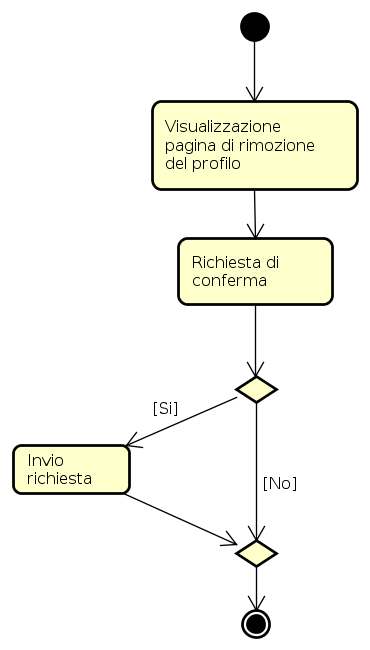
\includegraphics[height=12cm]{res/sections/backend/activities/rimuoviProfilo.png}
\caption{Rimozione dell'utente}
\end{center}
\end{figure}
L'utente autenticato, dopo aver visualizzato la pagina con i suoi dati personali, può decidere di cancellarsi da MaaS. Viene proposta una richiesta di conferma per evitare eliminazioni accidentali. Se la richiesta viene confermata, l'utente è rimosso da MaaS.
\subsubsection{Operazioni su specifiche DSL}
\begin{figure}[H]
\begin{center}
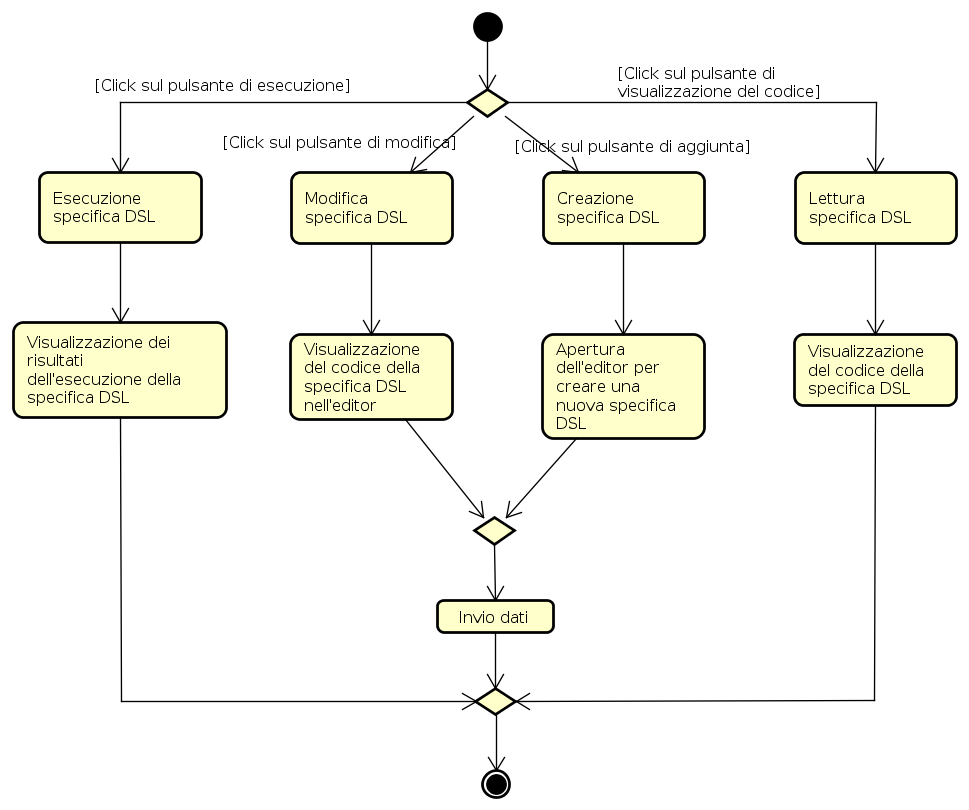
\includegraphics[height=12cm]{res/sections/backend/activities/operazioniDSL.png}
\caption{Operazioni su specifiche DSL}
\end{center}
\end{figure}
Un utente autenticato può decidere di effettuare varie operazioni sulle specifiche DSL alle quali ha accesso; in particolare:
\begin{itemize}
\item eseguire una specifica DSL, e visualizzare il risultato in forma tabellare;
\item modificare una specifica DSL;
\item creare una specifica DSL;
\item leggere il codice della specifica DSL.
\end{itemize}
Le ultime tre operazioni coinvolgono l'editor fornito da MaaS.
\subsubsection{Operazioni sulla dashboard}
\begin{figure}[H]
\begin{center}
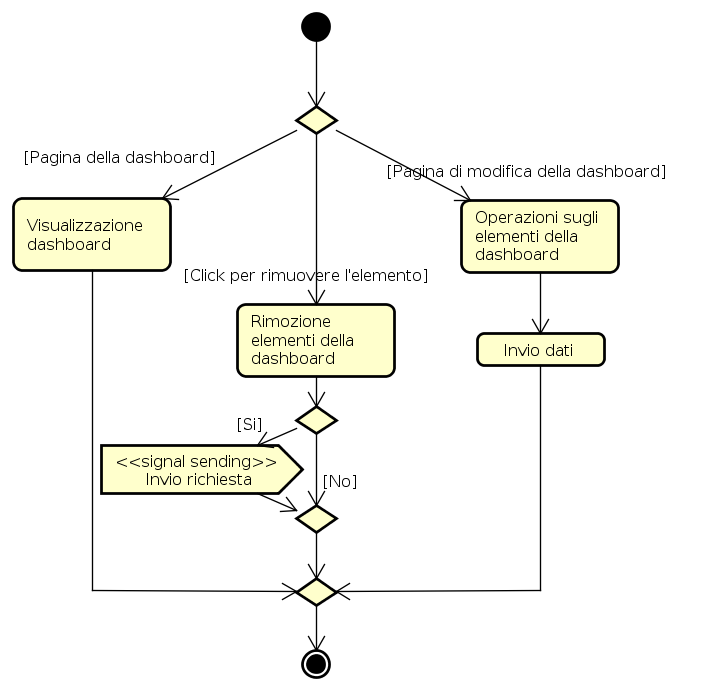
\includegraphics[height=12cm]{res/sections/backend/activities/operazioniDashboard.png}
\caption{Operazioni sulla dashboard}
\end{center}
\end{figure}
Un utente autenticato può decidere di effettuare varie operazioni sulla propria dashboard; in particolare:
\begin{itemize}
\item visualizzare gli elementi;
\item rimuovere degli elementi;
\item modificare degli elementi.
\end{itemize}
La rimozione degli elementi viene effettuata dopo una richiesta di conferma.
\paragraph{Visualizzazione elementi della dashboard} \mbox{} \\
\begin{figure}[H]
\begin{center}
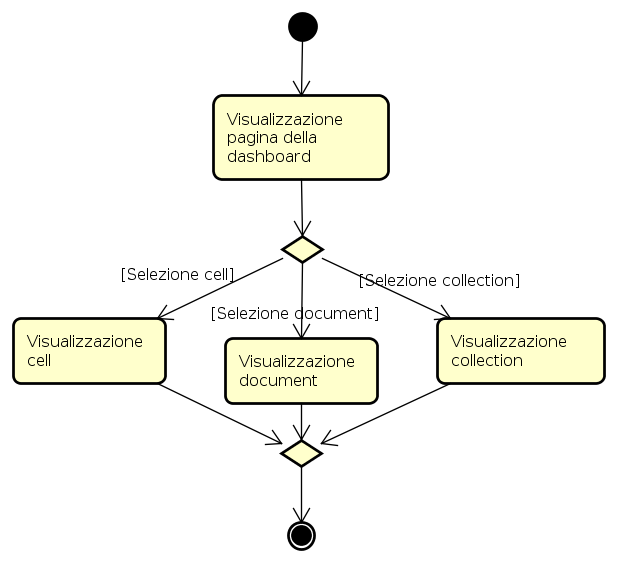
\includegraphics[height=12cm]{res/sections/backend/activities/visualizzazioneElementDashboard.png}
\caption{Visualizzazione elementi della dashboard}
\end{center}
\end{figure}
La dashboard si compone di cell, document e collection. Un utente può decidere di visualizzare questi elementi.
\paragraph{Modifica elementi della dashboard} \mbox{} \\
\begin{figure}[H]
\begin{center}
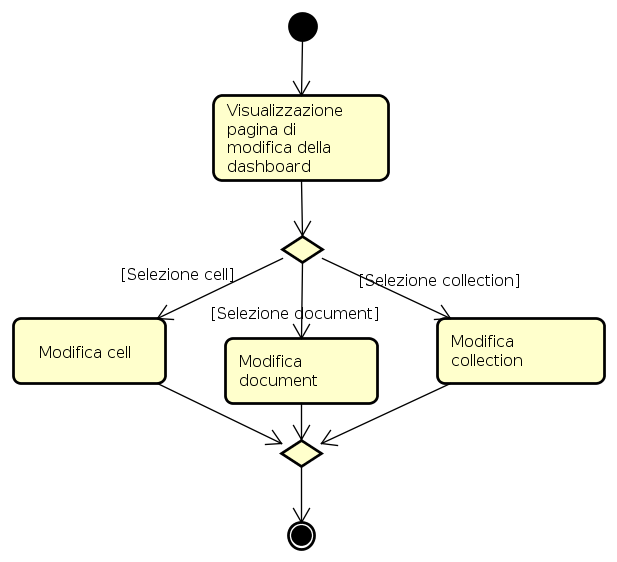
\includegraphics[height=12cm]{res/sections/backend/activities/modificaElementDashboard.png}
\caption{Modifica elementi della dashboard}
\end{center}
\end{figure}
La dashboard si compone di cell, document e collection. Un utente può decidere di modificare uno di questi tre elementi.
\subparagraph{Modifica cell} \mbox{} \\
\begin{figure}[H]
\begin{center}
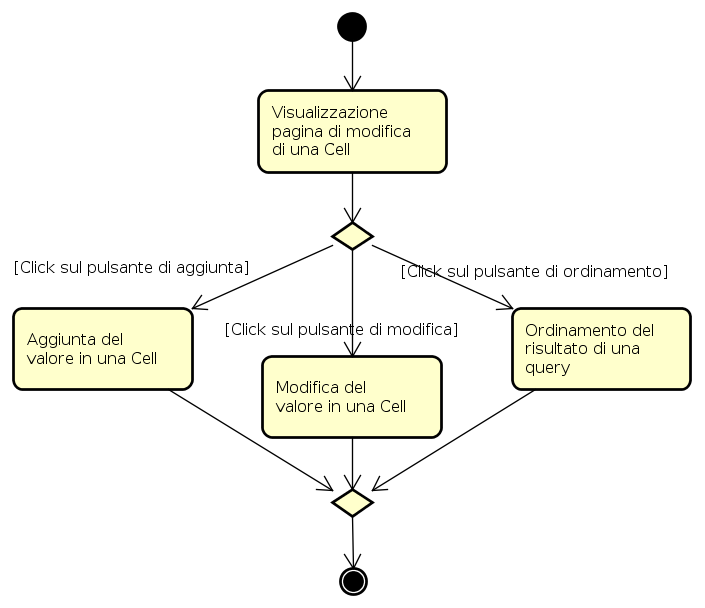
\includegraphics[height=12cm]{res/sections/backend/activities/modificaCell.png}
\caption{Modifica cell}
\end{center}
\end{figure}
Durante la modifica di una cell, l'utente autenticato può fare una delle seguenti tre operazioni:
\begin{itemize}
\item aggiungere un valore;
\item modificare un valore;
\item ordinare il risultato di una query.
\end{itemize}
\subparagraph{Gestione document} \mbox{} \\
\begin{figure}[H]
\begin{center}
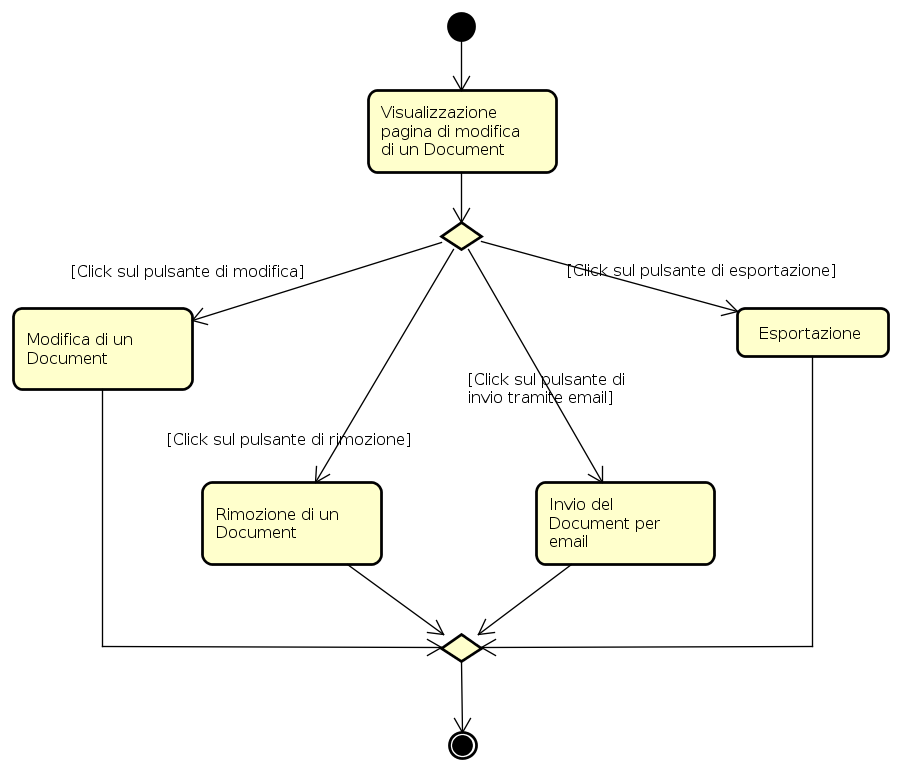
\includegraphics[height=12cm]{res/sections/backend/activities/modificaDocument.png}
\caption{Modifica document}
\end{center}
\end{figure}
Durante la gestione di un document, l'utente autenticato può fare una delle seguenti quattro operazioni:
\begin{itemize}
\item modificarlo;
\item rimuoverlo;
\item inviarlo per email;
\item esportarlo e salvarlo in locale.
\end{itemize}
\subparagraph{Gestione collection} \mbox{} \\
\begin{figure}[H]
\begin{center}
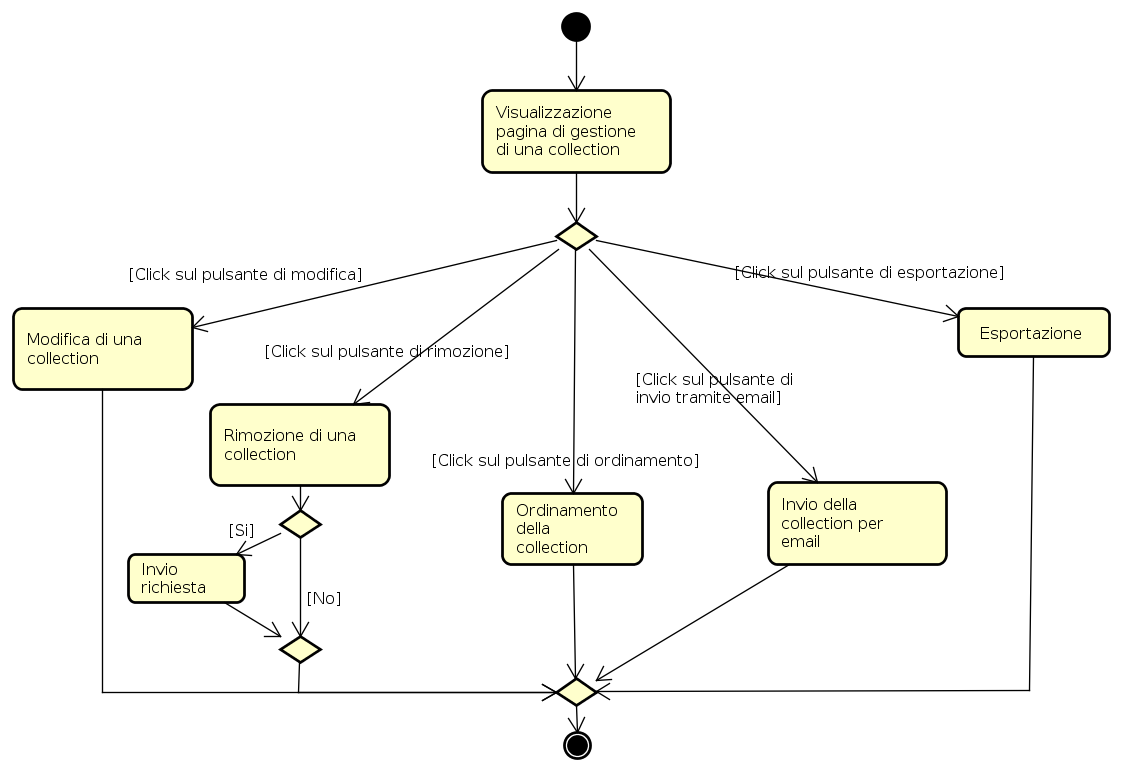
\includegraphics[width=16cm]{res/sections/backend/activities/gestioneCollection.png}
\caption{Gestione collection}
\end{center}
\end{figure}
Durante la gestione di una collection, l'utente autenticato può fare una delle seguenti cinque operazioni:
\begin{itemize}
\item modificarla;
\item rimuoverla;
\item ordinare i dati contenuti;
\item inviarla per email;
\item esportarla e salvarla in locale.
\end{itemize}
\subsubsection{Operazioni sui permessi degli utenti}
\begin{figure}[H]
\begin{center}
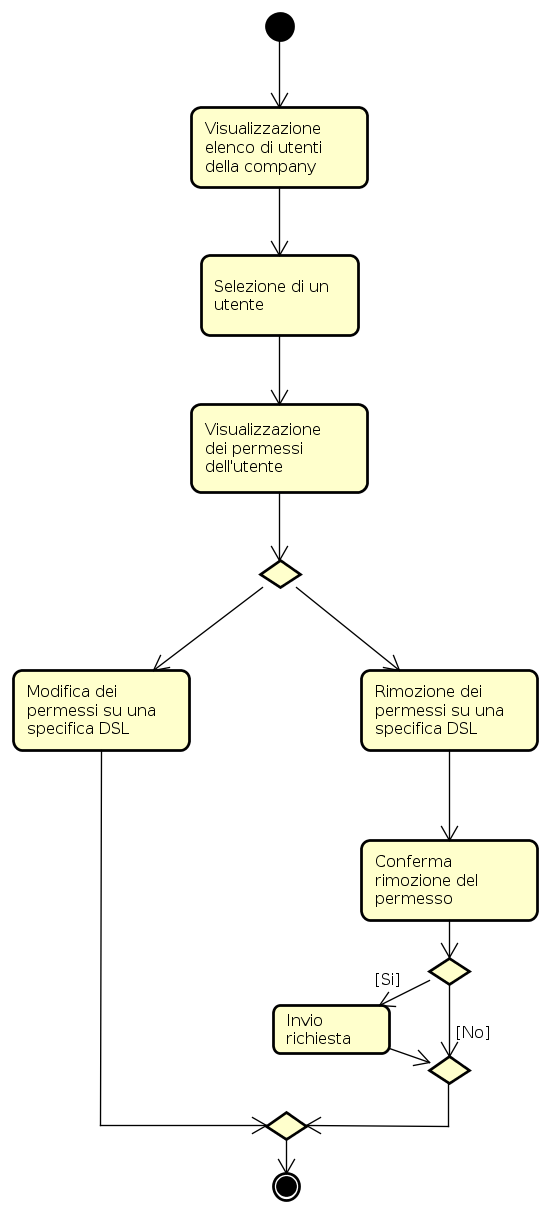
\includegraphics[height=12cm]{res/sections/backend/activities/operazioniSuUtenti.png}
\caption{Operazioni sui permessi degli utenti}
\end{center}
\end{figure}
Un utente autenticato, admin o owner, può modificare, o rimuovere, i permessi di un utente della stessa company.
\subsubsection{Operazioni sugli utenti}
\begin{figure}[H]
\begin{center}
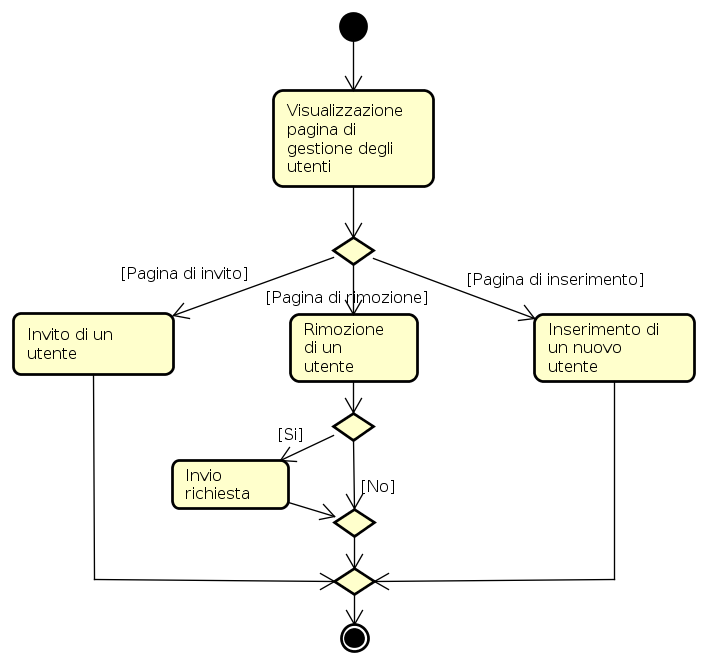
\includegraphics[height=12cm]{res/sections/backend/activities/gestioneUtenti.png}
\caption{Operazioni sugli utenti}
\end{center}
\end{figure}
Un utente autenticato, admin o owner, può gestire gli utenti della company che gestisce. In particolare può:
\begin{itemize}
\item invitare un utente;
\item rimuovere un utente;
\item inserire un utente.
\end{itemize}
\paragraph{Invito utente} \mbox{} \\
\begin{figure}[H]
\begin{center}
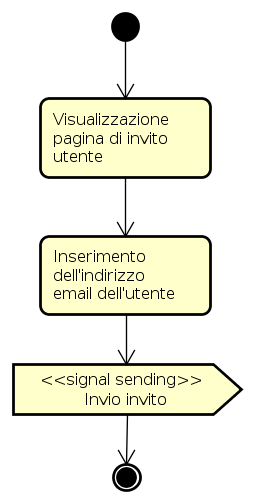
\includegraphics[height=12cm]{res/sections/backend/activities/invitoUtente.png}
\caption{Invito utente}
\end{center}
\end{figure}
Un utente autenticato, owner o admin, può invitare un nuovo utente nella propria company inserendo un indirizzo email ed inviando la richiesta tramite un pulsante presente nella pagina.
\paragraph{Inserimento utente} \mbox{} \\
\begin{figure}[H]
\begin{center}
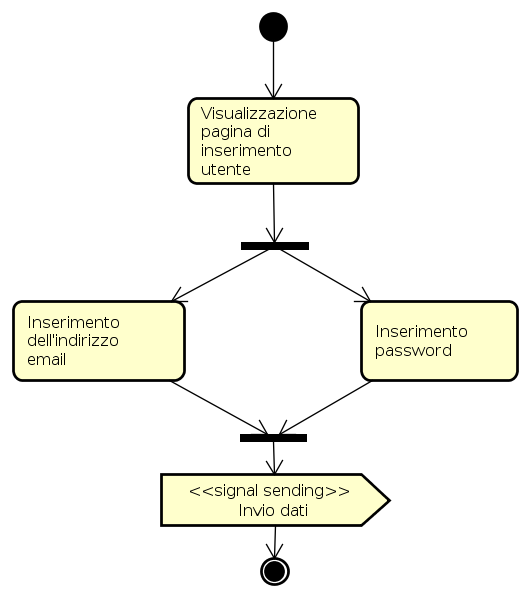
\includegraphics[height=12cm]{res/sections/backend/activities/inserimentoUtente.png}
\end{center}
\end{figure}
Un utente autenticato, owner o admin, può inserire manualmente un nuovo utente nella company senza prima invitarlo. Per farlo deve fornire indirizzo email e password del nuovo utente.
\subsubsection{Operazioni sui database}
\begin{figure}[H]
\begin{center}
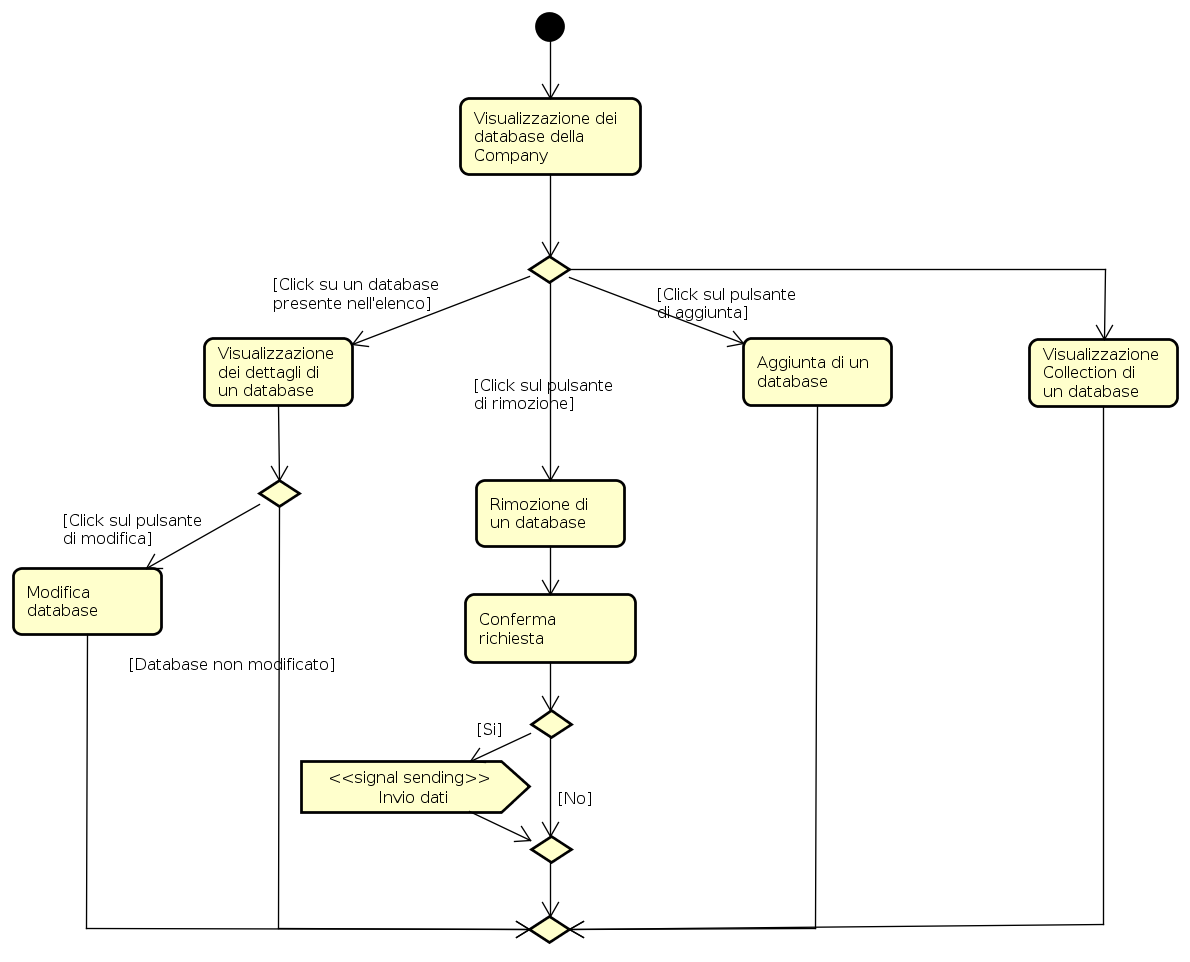
\includegraphics[height=12cm]{res/sections/backend/activities/gestioneDatabase.png}
\caption{Operazioni sui database della company}
\end{center}
\end{figure}
Un utente autenticato può visualizzare i database della company, e le collection di quel database, ai quali ha accesso. Gli admin e gli owner, invece, possono gestire i database registrati presso la company:
\begin{itemize}
\item modificando i dati di accesso e aggiungendo restrizioni sulle collections visibili ai member;
\item aggiungendo un database;
\item rimuovendo un database.
\end{itemize} 
\paragraph{Modifica database} \mbox{} \\
\begin{figure}[H]
\begin{center}
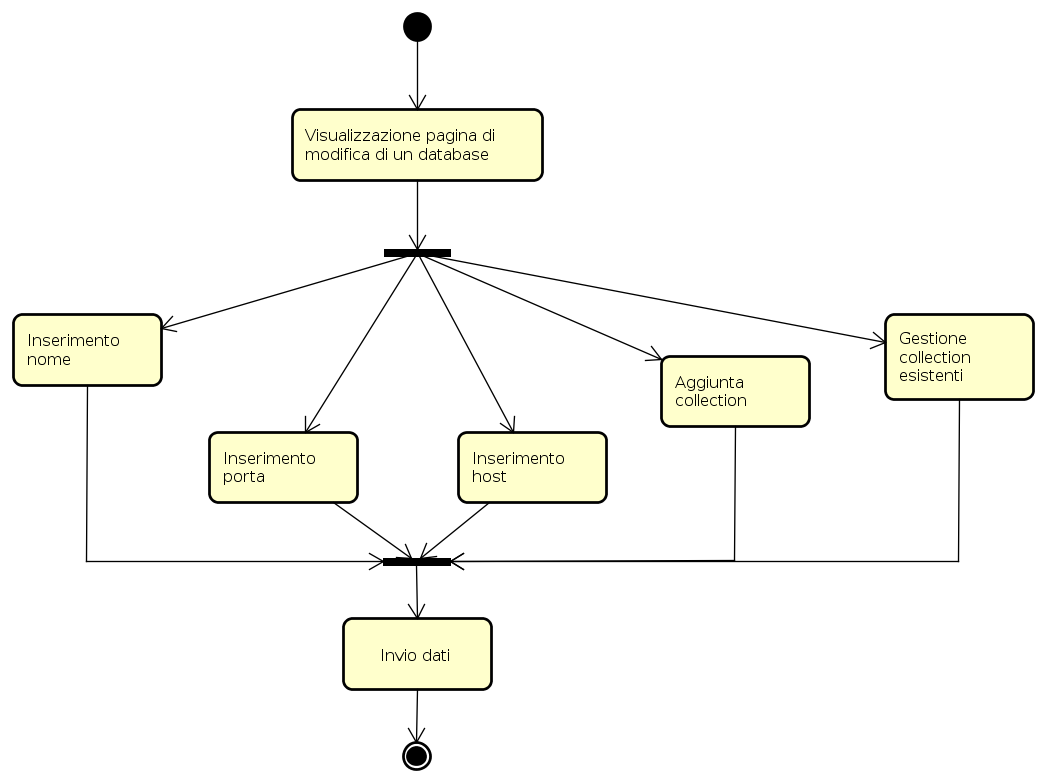
\includegraphics[height=12cm]{res/sections/backend/activities/modificaDatabase.png}
\end{center}
\end{figure}
Un admin o un owner può modificare un database della propria company. In particolare deve fornire:
\begin{itemize}
\item nome;
\item host;
\item porta di accesso;
\end{itemize}
Inoltre può aggiungere, rimuovere o modificare restrizioni sulle collections di quel database.
\subparagraph{Aggiunta collection} \mbox{} \\
\begin{figure}[H]
\begin{center}
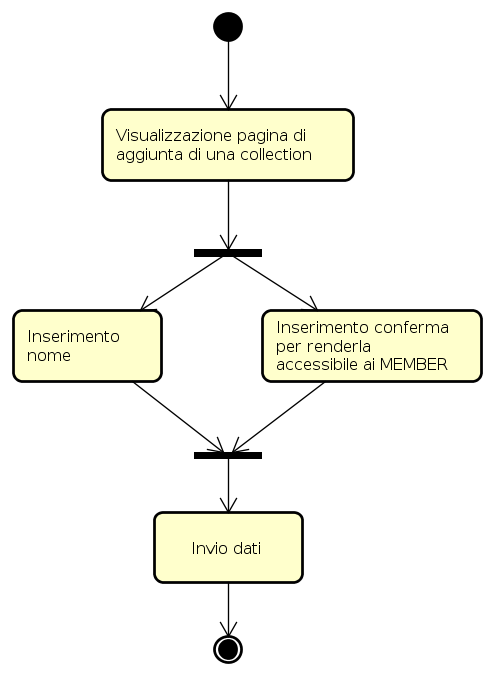
\includegraphics[height=12cm]{res/sections/backend/activities/aggiuntaDatiCollection.png}
\end{center}
\end{figure}
Un admin o un owner può decidere se rendere una nuova collection visibile ai members della company completando il form di aggiunta di una collection.
\subparagraph{Gestione collection} \mbox{} \\
\begin{figure}[H]
\begin{center}
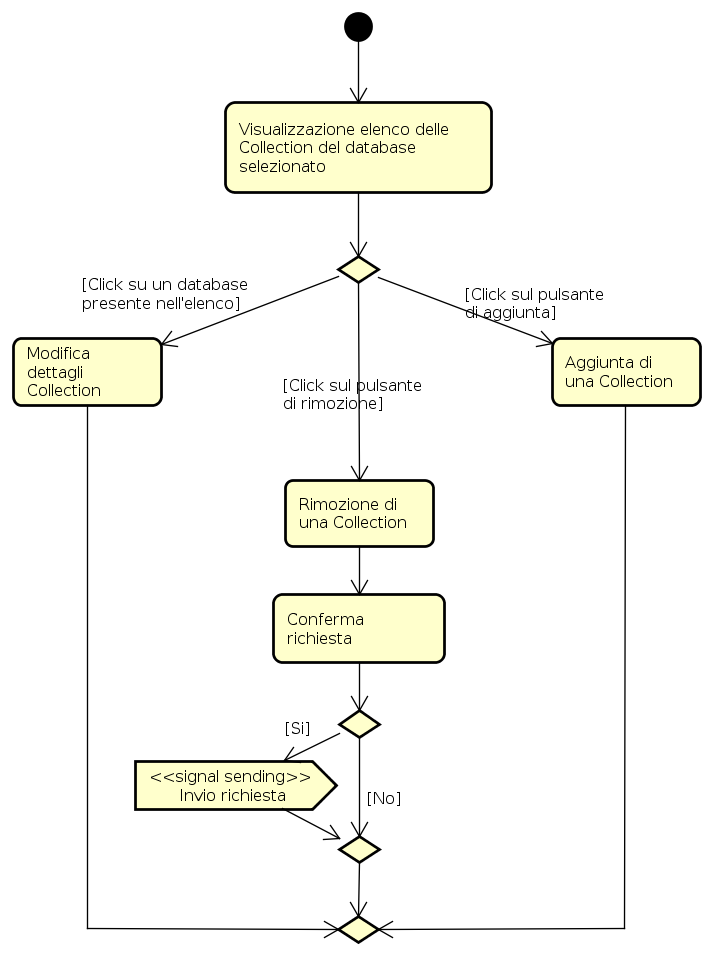
\includegraphics[height=12cm]{res/sections/backend/activities/gestioneCollectionAdmin.png}
\end{center}
\end{figure}
Un admin o un owner può modificare le regole di accesso e rimuovere le collection esistenti.
\subparagraph{Modifica collection} \mbox{} \\
\begin{figure}[H]
\begin{center}
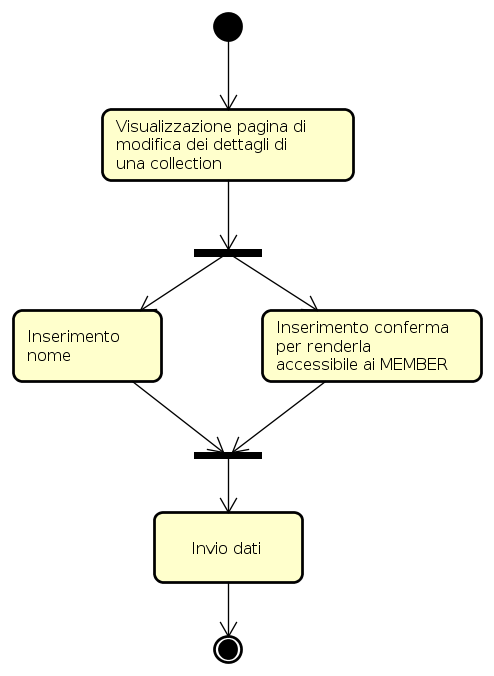
\includegraphics[height=12cm]{res/sections/backend/activities/modificaDatiCollection.png}
\end{center}
\end{figure}
Un admin o un owner può decidere se rendere una collection già esistente visibile ai members della company completando il form di modifica di una collection.
\paragraph{Aggiunta database} \mbox{} \\
\begin{figure}[H]
\begin{center}
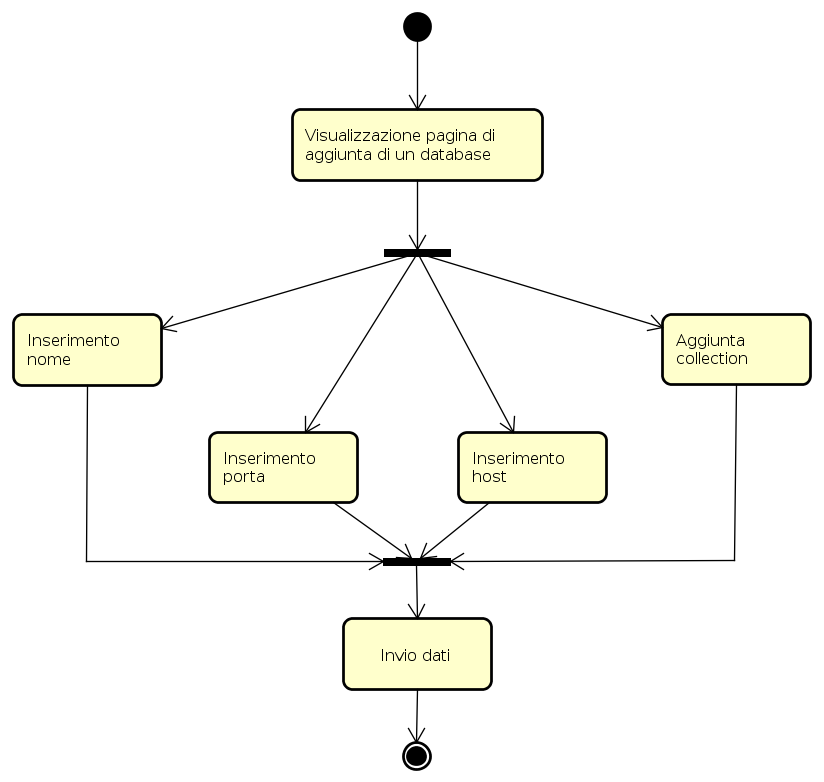
\includegraphics[height=12cm]{res/sections/backend/activities/aggiuntaDatabase.png}
\end{center}
\end{figure}
Un admin o un owner può aggiungere un database nella propria company. In particolare deve fornire:
\begin{itemize}
\item nome;
\item host;
\item porta di accesso;
\end{itemize}
Inoltre può aggiungere collections nel database, e restrizioni su di esse.
\subsection{Super Admin}
\begin{figure}[H]
\begin{center}
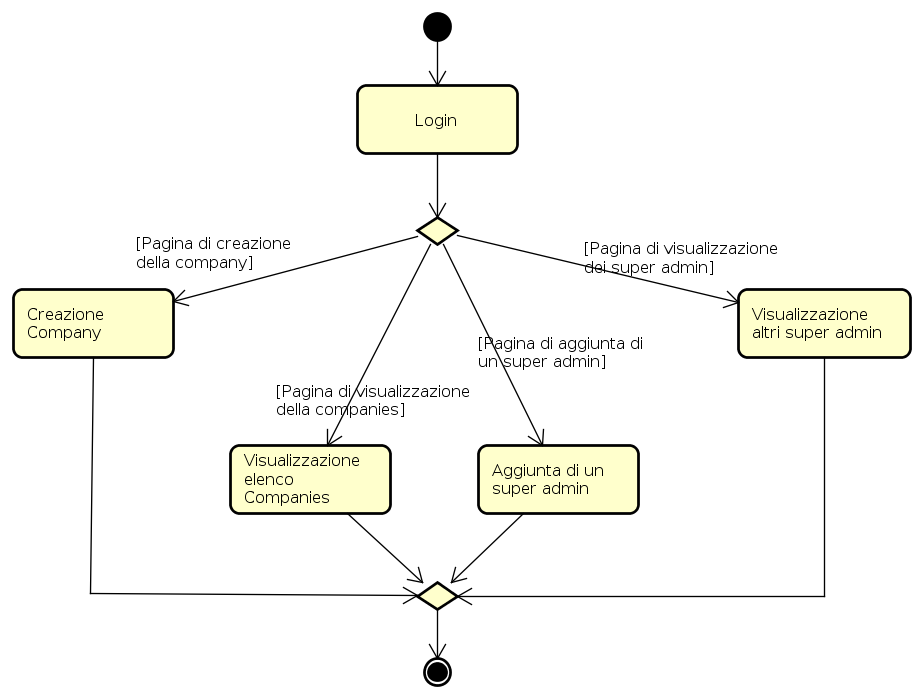
\includegraphics[height=12cm]{res/sections/backend/activities/principaliSuperAdmin.png}
\caption{Attività principali per il super admin}
\end{center}
\end{figure}
Dopo aver effettuato il login, il super admin può:
\begin{itemize}
\item creare una company;
\item visualizzare l'elenco delle company registrate a MaaS;
\item aggiungere un altro super admin;
\item visualizzare i dettagli sugli altri super admin.
\end{itemize}
\subsubsection{Creazione company}
\begin{figure}[H]
\begin{center}
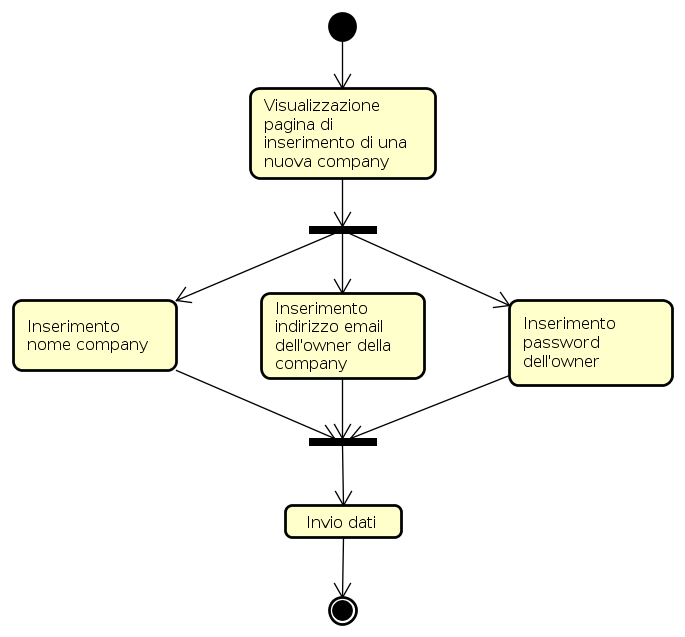
\includegraphics[height=12cm]{res/sections/backend/activities/creazioneCompanySA.png}
\caption{Creazione company}
\end{center}
\end{figure}
Il super admin che crea una company deve fornire i dati dell'utente che verrà registrato come owner. È pertanto necessario fornire, durante la procedura di creazione, l'indirizzo email e la password del nuovo utente, oltre che il nome della company stessa.
\subsubsection{Visualizzazione elenco companies}
\begin{figure}[H]
\begin{center}
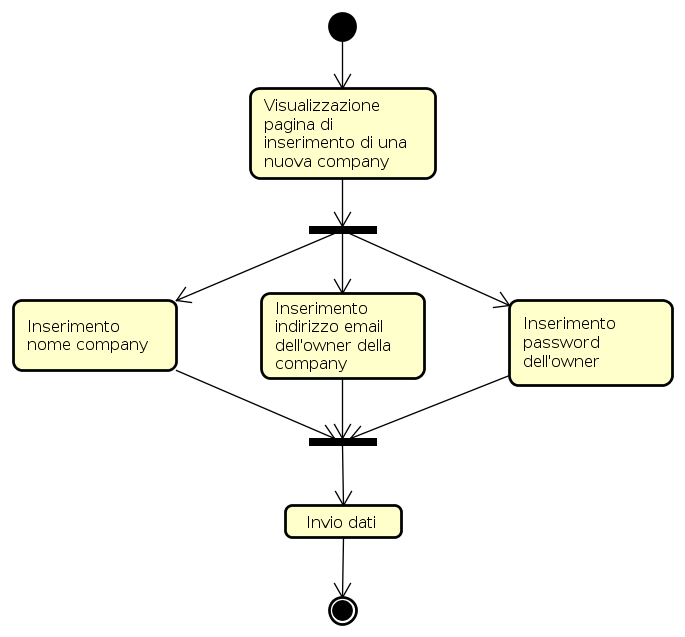
\includegraphics[height=12cm]{res/sections/backend/activities/creazioneCompanySA.png}
\caption{Visualizzazione elenco companies}
\end{center}
\end{figure}
Il super admin può visualizzare tutte le company presenti in MaaS, ed eseguire varie operazioni su di esse:
\begin{itemize}
\item modificare i dati della company;
\item aggiungere un utente;
\item visualizzarne gli utenti.
\end{itemize}
\paragraph{Modifica company} \mbox{} \\
\begin{figure}[H]
\begin{center}
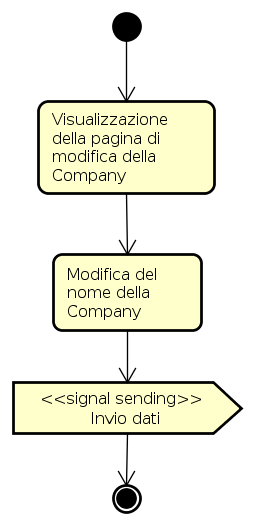
\includegraphics[height=12cm]{res/sections/backend/activities/modificaCompanySA.png}
\caption{Modifica dei dati di una company}
\end{center}
\end{figure}
Il super admin può modificare il nome di una company inserendo il nuovo nome in una casella di testo ed inviando la richiesta di aggiornamento tramite un pulsante presente sulla pagina.
\paragraph{Aggiunta utente} \mbox{} \\
\begin{figure}[H]
\begin{center}
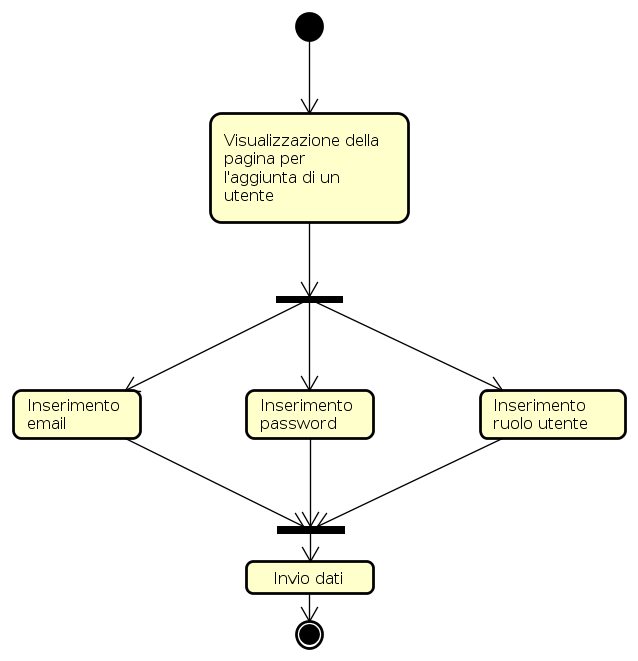
\includegraphics[height=12cm]{res/sections/backend/activities/aggiuntaUtenteSA.png}
\caption{Aggiunta di un utente alla company}
\end{center}
\end{figure}
Il super admin può aggiungere un utente alla company selezionata inserendone indirizzo email, password e ruolo. 
\paragraph{Visualizzazione utenti della company} \mbox{} \\
\begin{figure}[H]
\begin{center}
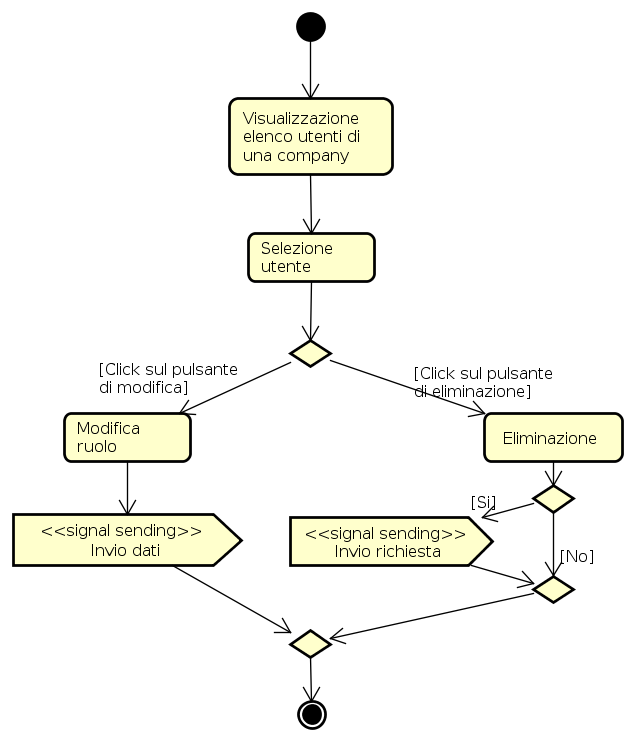
\includegraphics[height=12cm]{res/sections/backend/activities/operazioniUtentiSA.png}
\caption{Visualizzazione utenti della company}
\end{center}
\end{figure}
Una volta visualizato l'elenco degli utenti iscritti alla comapny, il super admin può modificare il ruolo di un utente o di rimuoverlo. Nel secondo caso è richiesta una conferma, per evitare eliminazioni accidentali.
\subsubsection{Aggiunta di un super admin}
\begin{figure}[H]
\begin{center}
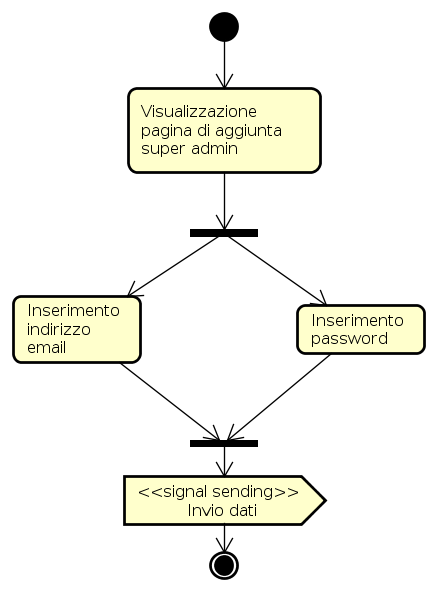
\includegraphics[height=12cm]{res/sections/backend/activities/aggiuntaSuperAdmin.png}
\caption{Aggiunta super admin}
\end{center}
\end{figure}
Il super admin può visualizzare tutte le company presenti in MaaS, ed eseguire varie Il super admin può inserire un altro super admin all'intero di MaaS, per farlo è necessario fornirne indirizzo email e password, ed inviare i dati attraverso un apposito pulsante.
\subsubsection{Visualizzazione dettagli di un super admin}
\begin{figure}[H]
\begin{center}
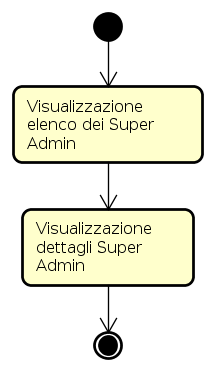
\includegraphics[height=12cm]{res/sections/backend/activities/visualizzazioneDettagliSuperAdminSA.png}
\caption{Visualizzazione altri super admins}
\end{center}
\end{figure}
Il super admin può visualizzare i dettagli sugli altri super admin a partire dalla pagina di elenco dei super admin presenti in MaaS. Per fare questo è sufficiente fare click sul super admin del quale si vogliono visualizzare i dettagli.